\subsubsection{08.02.15}
\begin{enumerate}
	
	\item Время начала и окончания собрания: 12:30 - 18:00.
	
	\item Цели собрания: 
	\begin{enumerate}
		
		\item Модернизировать МЗК таким образом, чтобы он не терял подвижную корзину на большой скорости.
		
		\item Написать программу автономного периода для старта с пандуса.
		
	\end{enumerate}

	\item Проделанная работа:
	\begin{enumerate}
		
		\item Для того, чтобы МЗК не открывался и не терял подвижную корзину, было решено установить на него два сервопривода вместо одного. Для того, чтобы сервоприводы поворачивались синхронно, они были сначала установлены в положения 0${\textdegree}$ и 180${\textdegree}$ соответственно таким образом, что их крепления располагались ровно друг напротив друга и лишь потом закреплены. После этого функция управления МЗК была изменена под 2 сервопривода. Испытания захвата прошли успешно, корзина не терялась роботом на любой скорости.
		\begin{figure}[H]
			\begin{minipage}[h]{0.2\linewidth}
				\center  
			\end{minipage}
			\begin{minipage}[h]{0.6\linewidth}
				\center{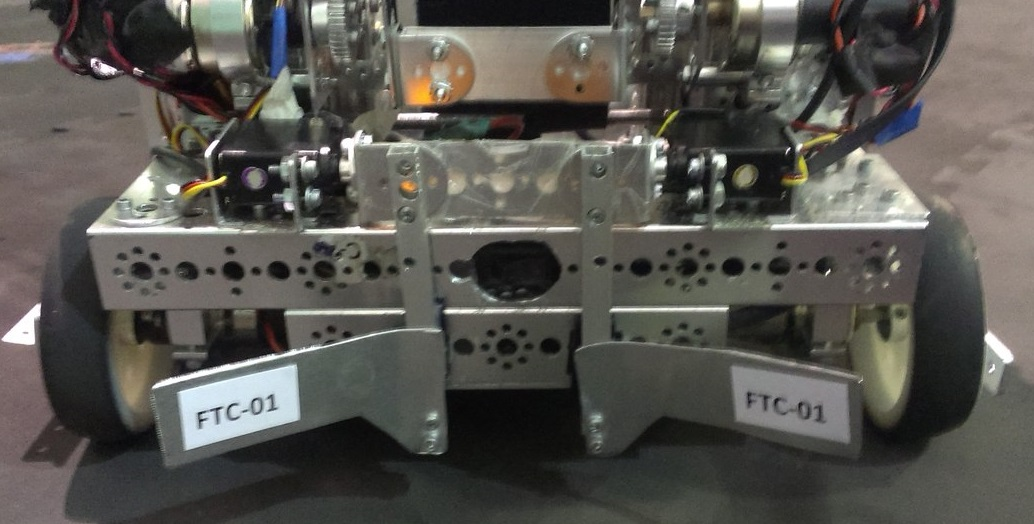
\includegraphics[scale=0.25]{days/08.02.15/images/01}}
				\caption{МЗК с двумя сервоприводами}
			\end{minipage}
		\end{figure}
		
		\item Программа автономного периода с пандуса была полностью написана. Стратегия автономного периода осталась прежней (съезд, закидывание мячей в корзины 60 и 90 см, захват обеих корзин и доставка их в зону парковки). Для того, чтобы программа могла работать на соревнованиях, необходимо только подкорректировать значения поворотов под силу трения соревновательного поля.

	\end{enumerate}
	
	\item Итоги собрания:
	\begin{enumerate}
		
		\item Проблема с недостаточной мощностью механизма захвата корзин устранена.
		
		\item Программа автономного периода при старте с пандуса написана.
		
	\end{enumerate}
	
	\item Задачи для последующих собраний:
	\begin{enumerate}
		
		\item Продолжить тренировки в управлении роботом.
		
		\item Реализовать защиту колес от наезда на мячи и палку-упор.
			
	\end{enumerate}
\end{enumerate}
\fillpage
